\documentclass[conference]{IEEEtran}
\IEEEoverridecommandlockouts
\usepackage{cite}
\usepackage{tabularx}
\usepackage{amsmath,amssymb,amsfonts}
\usepackage{graphicx}
\usepackage{textcomp}
\usepackage{xcolor}
\usepackage{url} % Added for better URL formatting
\usepackage{caption} % Added for subfigures if needed and figure notes
\usepackage{algpseudocode}
\usepackage{pgfplots}
\pgfplotsset{compat=1.18} % Gunakan versi terbaru yang Anda miliki

\def\BibTeX{{\rm B\kern-.05em{\sc i\kern-.025em b}\kern-.08em
    T\kern-.1667em\lower.7ex\hbox{E}\kern-.125emX}}
\begin{document}

%\title{\textbf{Analisis Penentuan Ketinggian Awal Air dalam Tangki Silinder Menggunakan Metode Numerik}}
\title{\textbf{Pembuktian \textit{Bisection Method} dalam Perhitungan Ketinggian Awal Air pada Tangki (\textit{Bernoulli})}}

\author{
\IEEEauthorblockN{Bonifasius Raditya Pandu Hendrianto}
\IEEEauthorblockA{\textit{Teknik Komputer (2306242350)} \\
\textit{Universitas Indonesia}\\
Depok, Indonesia \\
radityahendrianto@gmail.com}
}

\maketitle

\begin{abstract}
Penentuan parameter aliran fluida merupakan aspek krusial dalam berbagai aplikasi rekayasa. Studi ini berfokus pada penentuan ketinggian awal air ($H$) dalam sebuah tangki silinder yang mengalir melalui pipa panjang. Kecepatan air keluar ($v$) dari sistem ini dapat dihitung menggunakan persamaan yang melibatkan $H$, panjang pipa ($L$), waktu ($t$), dan percepatan gravitasi ($g$). Penelitian ini bertujuan untuk menerapkan dan membandingkan tiga metode numerik pencarian akar — metode grafis, \textit{bisecton method} (bisection), dan metode posisi palsu (false position) — untuk menentukan nilai $H$ yang memenuhi kondisi aliran tertentu. Hasil dari setiap metode akan dianalisis untuk mengevaluasi akurasi dan efisiensinya dalam menyelesaikan permasalahan ini, dengan kriteria penghentian $\epsilon_s = 1\%$.
\end{abstract}

\begin{IEEEkeywords}
KEYWORD: \\
ketinggian awal, aliran pipa, metode grafis, \textit{bisecton method}, metode posisi palsu, numerik, pencarian akar
\end{IEEEkeywords}

\section{PENDAHULUAN}

Dalam disiplin ilmu mekanika fluida, analisis aliran dari tangki penyimpanan melalui pipa merupakan salah satu problem fundamental dengan aplikasi yang luas, mulai dari sistem irigasi hingga proses industri. Salah satu parameter penting dalam analisis tersebut adalah ketinggian awal ($H_0$) fluida dalam tangki, karena parameter ini mempengaruhi kecepatan aliran keluar. Persamaan yang menggambarkan fenomena ini seringkali bersifat non-linear dan transenden, sehingga penyelesaian analitik untuk mencari parameter tertentu seperti ketinggian awal menjadi tidak praktis atau bahkan tidak mungkin dilakukan.

Tujuan utama dari penelitian ini adalah untuk mendemonstrasikan penerapan \textit{bisecton method} secara sistematis dalam menemukan solusi numerik untuk permasalahan aliran fluida yang diberikan. Untuk memfokuskan analisis, studi ini menggunakan serangkaian parameter yang telah ditetapkan: kecepatan target air adalah $v = 4 \, \text{m/s}$, panjang pipa $L = 5 \, \text{m}$, dan waktu $t = 3 \, \text{s}$. Implementasi \textit{bisecton method} akan dilakukan dengan menggunakan interval awal tebakan $[0, 2]$ meter dan kriteria penghentian berupa galat relatif perkiraan ($\epsilon_a$) yang lebih kecil dari $1\%$.

\section{STUDI LITERATUR}
Dinamika fluida adalah cabang dari mekanika fluida yang mempelajari bagaimana fluida (cairan dan gas) bergerak serta gaya yang bekerja padanya. Studi ini sangat penting dalam berbagai aplikasi rekayasa, mulai dari desain pesawat hingga sistem perpipaan. Prinsip fundamental yang mendasari dinamika fluida adalah hukum kekekalan massa, momentum, dan energi. Dari prinsip-prinsip ini, diturunkan persamaan-persamaan yang menggambarkan hubungan antara properti fluida seperti tekanan, kecepatan, dan ketinggian. Salah satu persamaan paling terkenal dalam dinamika fluida adalah Persamaan Bernoulli, yang menghubungkan energi kinetik, energi potensial, dan energi aliran fluida di sepanjang garis aliran. Persamaan ini menjadi dasar untuk memahami fenomena seperti gaya angkat pada sayap pesawat dan aliran air dalam pipa.

Salah satu aplikasi langsung dari Prinsip Bernoulli adalah Hukum Torricelli. Hukum ini, yang dirumuskan oleh Evangelista Torricelli, secara spesifik menjelaskan kecepatan aliran keluar (efluks) suatu fluida dari sebuah lubang kecil pada sebuah wadah atau tangki. Dalam kondisi ideal, di mana lubang dianggap kecil dibandingkan luas penampang tangki dan viskositas diabaikan, hukum ini menyatakan bahwa kecepatan aliran keluar, $v$, sama dengan kecepatan yang akan diperoleh sebuah benda jika jatuh bebas dari ketinggian $h$, yaitu ketinggian permukaan fluida di atas lubang. Secara matematis, hukum ini dinyatakan sebagai $v = \sqrt{2gh}$, dengan $g$ adalah percepatan gravitasi. Hukum ini memberikan fondasi teoretis yang kuat untuk menganalisis sistem aliran sederhana, seperti yang digambarkan pada studi kasus ini.

Namun, Hukum Torricelli merupakan model ideal. Dalam sistem nyata yang melibatkan pipa panjang, faktor-faktor seperti gesekan (friksi) dan efek transien (perubahan seiring waktu) saat fluida mulai bergerak menjadi signifikan. 

\begin{figure}[htbp]
  \centering
  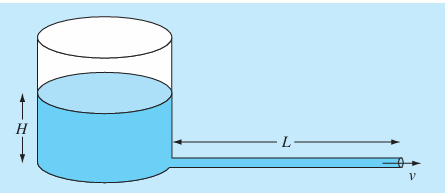
\includegraphics[width=\columnwidth]{src/5.15.png}
  \caption{Diagram skematik sistem tangki silinder dan pipa pembuangan.}
  \label{fig:sistem_tangki}
\end{figure}

\begin{equation}
v = \sqrt{2gH} \tanh\left(\frac{\sqrt{2gH}}{2L}t\right)
\label{eq:kecepatan_air}
\end{equation}
Untuk mencari nilai ketinggian awal air ($H$) yang diperlukan untuk mencapai kecepatan aliran tertentu ($v$), kita perlu menyelesaikan persamaan berikut:
\begin{equation}
    f(H) = \sqrt{2gH} \tanh\left(\frac{\sqrt{2gH}}{2L}t\right) - v
    \label{eq:bernoulli_inverse}
\end{equation}
dimana:
\begin{itemize}
    \item $H$ adalah ketinggian air (m) 
    \item $g$ adalah percepatan gravitasi ($9.81 \text{ m/s}^2$) 
    \item $v$ adalah kecepatan aliran air (m/s) 
    \item $L$ adalah panjang pipa (m) 
    \item $t$ adalah waktu yang telah berlalu (s) 
\end{itemize}
Fungsi tangen hiperbolik ($\tanh$) dalam persamaan ini merepresentasikan bagaimana kecepatan aliran air ($v$) mempengaruhi ketinggian air ($H$) secara bertahap. Metode numerik diperlukan untuk menyelesaikan persamaan ini karena sifat non-linear dari fungsi $\tanh$ yang membuat solusi analitik sulit dicapai. Oleh karena itu, metode pencarian akar seperti \textit{bisection method} akan digunakan untuk menemukan nilai $H$ yang memenuhi persamaan tersebut. \\

\textit{Bisection method} merupakan metode numerik yang digunakan untuk menemukan akar dari suatu fungsi dengan cara membagi interval yang mengandung akar menjadi dua bagian dan memilih bagian yang mengandung akar. Metode ini sangat efektif untuk fungsi kontinu dan dapat menjamin konvergensi ke akar yang diinginkan jika interval awal dipilih dengan benar. Metode ini dimulai dengan memilih dua tebakan awal, $x_l$ (batas bawah) dan $x_u$ (batas atas), yang harus mengurung akar. Kemudian, titik tengah dari interval tersebut dihitung sebagai estimasi awal akar. Proses ini diulang dengan memperbarui interval berdasarkan tanda dari fungsi pada titik tengah hingga galat relatif perkiraan ($\epsilon_a$) mencapai kriteria penghentian yang ditentukan.

\section{DATA PENGUJIAN}
Terdapat beberapa variabel yang digunakan dalam perhitungan numerik \textit{bisection method ini}. Parameter waktu (t), panjang saluran (L), dan percepatan gravitasi akan berperan sebagai variabel kontrol karena nilainya sudah ditetapkan diawal. Parameter yang dijaga konstan selama simulasi adalah:
\begin{itemize}
    \item Kecepatan Aliran Air ($v$) sebesar $4.00 \, \text{m/s}$.
    \item Percepatan gravitasi ($g$) sebesar $9.81 \, \text{m/s}^2$.
    \item Panjang saluran ($L$) sepanjang $5.00 \, \text{m}$.
    \item Waktu yang telah berlalu ($t$) selama $3.00 \, \text{s}$.
\end{itemize}
Hasil dari perhitungan numerik ini adalah perbandingan perhitungan numerik \textit{bisection method} dengan rumus prinsip bernoulli untuk mencari nilai H (m) sebagai variabel terikat. Rumus yang digunakan mengandung unsur prinsip bernoulli. 

\section{METODE PENYELESAIAN}

Metode yang dipakai untuk menyelesaikan permasalahan ini adalah \textbf{\textit{bisecton method} (bisection method)}. Metode ini merupakan metode pencarian akar yang didasarkan pada teorema nilai antara. Prosesnya dimulai dengan menentukan dua tebakan awal, $x_l$ (batas bawah) dan $x_u$ (batas atas), yang harus mengurung akar, yang berarti perkalian nilai fungsi pada kedua titik tersebut harus negatif ($f(x_l)f(x_u) < 0$). Estimasi akar berikutnya, $x_r$, dihitung sebagai titik tengah interval:
\begin{equation}
    x_r = \frac{x_l + x_u}{2}
\end{equation}
Interval kemudian diperbarui untuk iterasi selanjutnya. Galat relatif perkiraan ($\epsilon_a$) dihitung untuk mengukur perubahan antara estimasi akar yang baru dan yang sebelumnya, menggunakan rumus:
\begin{equation}
    \epsilon_a = \left|\frac{x_{r}^{\text{baru}} - x_{r}^{\text{lama}}}{x_{r}^{\text{baru}}}\right| \times 100\%
\end{equation} 
Iterasi akan berhenti ketika nilai $\epsilon_a$ lebih kecil atau sama dengan kriteria penghentian yang ditentukan ($\epsilon_s$).

Nilai dari $x_l$ dan $x_u$ awal ditentukan dari tebakan awal yang masuk akal. Nilai setelahny a akan dihitung berdasarkan fungsi $f(H)$ yang telah didefinisikan sebelumnya. Jika $f(x_l)$ dan $f(x_r)$ memiliki tanda yang berbeda atau negatif, maka akar terletak di antara $x_l$ dan $x_r$, sehingga kita akan memperbarui batas atas ($x_u$) menjadi $x_r$. Sebaliknya, jika tanda dari $f(x_l)$ dan $f(x_r)$ sama atau positif, maka akar terletak di antara $x_r$ dan $x_u$, sehingga kita akan memperbarui batas bawah ($x_l$) menjadi $x_r$. Proses ini diulang hingga galat relatif perkiraan mencapai kriteria penghentian yang telah ditentukan. Pada kasus ini, $\epsilon_s = 1\%$. 

Berikut merupakan pseudocode untuk pengimplementasian \textit{bisection method}:
\begin{flushleft}
\begin{algorithmic}[1]
    \State Definisikan fungsi $f(H) \gets \sqrt{2gH} \tanh\left(\frac{\sqrt{2gH}}{2L}t\right) - v$.
    \State Inisialisasi parameter yang diperlukan: batas awal $x_l$ dan $x_u$, serta kriteria berhenti $\epsilon_s$.
    \State Inisialisasi variabel penyimpan: $H_0^{\text{lama}} \gets 0$.
    \While{true}
        \State Hitung estimasi akar baru: $H_0 \gets \frac{x_l + x_u}{2}$.
        \State Hitung galat relatif perkiraan: $\epsilon_a \gets \left| (H_0 - H_0^{\text{lama}}) / H_0 \right| \times 100\%$.
        \If{$\epsilon_a \le \epsilon_s$}
            \State \textbf{break}
        \EndIf
        \If{$f(x_l) \cdot f(H_0) < 0$}
            \State Perbarui batas atas: $x_u \gets H_0$.
        \Else
            \State Perbarui batas bawah: $x_l \gets H_0$.
        \EndIf
        \State Simpan estimasi saat ini untuk iterasi berikutnya: $H_0^{\text{lama}} \gets H_0$.
    \EndWhile
    \State \Return $H_0$
\end{algorithmic}
\end{flushleft}

Setelah itu, dilakukan perhitungan untuk mencari nilai galat relatif $v_\text{numerik}$ perhitungan bernoulli menggunakan hasil dari \textit{bisection method} dari $v_\text{target}$ kita dapat menggunakan rumus:
\begin{equation}
\epsilon_r = \left| \frac{v_{\text{target}} - v_{\text{numerik}}}{v_{\text{target}}} \right| \times 100\%
\end{equation}


\section{DISKUSI DAN ANALISA HASIL EKSPERIMEN}
Hasil perhitungan numerik \textit{bisection method} akan dibandingkan dengan perhitungan nilai fungsi f(H) sehingga perbandingan tersebut akan menjadi tolak ukur dari keakuratan \textit{bisection method}. Dengan menggunakan \textit{bisection method}, kita akan mencari nilai ketinggian awal ($H$) yang diperlukan untuk mencapai kecepatan aliran $4 \, \text{m/s}$ dengan parameter sebagai berikut:
\begin{itemize}
    \item Fungsi target: $f(H) = \sqrt{2gH} \tanh\left(\frac{\sqrt{2gH}}{2L}t\right) - 4 = 0$
    \item Interval awal: $[x_l, x_u] = [0, 2]$
    \item Kriteria berhenti: $\epsilon_s = 1\%$
\end{itemize}
\begin{table}[htbp]
\centering
\caption{Hasil Iterasi \textit{bisection method} untuk Mencari H}
\label{tab:hasil_bisection}
\renewcommand{\arraystretch}{1.2}
\begin{tabular}{|c|c|c|c|r|c|}
\hline
\textbf{Iterasi} & $\boldsymbol{x_l}$ & $\boldsymbol{x_u}$ & $\boldsymbol{x_r}$ & \multicolumn{1}{c|}{$\boldsymbol{f(x_r)}$} & $\boldsymbol{\epsilon_a (\%)}$ \\
\hline
1 & 0.000000 & 2.000000 & 1.000000 & -0.15097 & - \\
2 & 1.000000 & 2.000000 & 1.500000 & 1.01452 & 33.33 \\
3 & 1.000000 & 1.500000 & 1.250000 & 0.46467 & 20.00 \\
4 & 1.000000 & 1.250000 & 1.125000 & 0.16543 & 11.11 \\
5 & 1.000000 & 1.125000 & 1.062500 & 0.00934 & 5.88  \\
6 & 1.000000 & 1.062500 & 1.031250 & -0.07026 & 3.03  \\
7 & 1.031250 & 1.062500 & 1.046875 & -0.03032 & 1.49  \\
8 & 1.046875 & 1.062500 & \textbf{1.054688} & -0.01046 & \textbf{0.74} \\
\hline
\end{tabular}
\end{table}
Nilai pada tabel ini didapat dari perhitungan iteratif menggunakan \textit{bisection method} dengan memasukan nilai kecepatan aliran yang diinginkan ($v = 4 \, \text{m/s}$) untuk mendapatkan nilai $H_0$ yang sesuai.

Berikut merupakan perhitungan setiap iterasi yang ada menggunakan \textit{bisection method} untuk mencari nilai ketinggian awal ($H$) yang diperlukan untuk mencapai kecepatan aliran $4 \, \text{m/s}$ dengan parameter awal sebagai berikut:
\begin{itemize}
    \item Fungsi target: $f(H) = \sqrt{2gH} \tanh\left(\frac{\sqrt{2gH}}{2L}t\right) - 4 = 0$
    \item Interval awal: $[x_l, x_u] = [0, 2]$
    \item Kriteria berhenti: $\epsilon_s = 1\%$
\end{itemize}
Iterasi ke-1 adalah nilai tengah dari interval 0 dan 2, yakni 1.0 sebagai nilai bagi dua.

Perhitungan untuk Iterasi ke-2:
\begin{enumerate}
    \item Identifikasi nilai $x_r$ yang relevan:
    \begin{itemize}
        \item $x_{r, \text{baru}}$ (dari iterasi ke-2) = \textbf{1.5}
        \item $x_{r, \text{lama}}$ (dari iterasi ke-1) = \textbf{1.0}
    \end{itemize}
    
    \item Masukkan ke dalam rumus:
    \begin{equation}
    \epsilon_a = \left| \frac{1.5 - 1.0}{1.5} \right| \times 100\%
    \end{equation}
    
    \item Selesaikan kalkulasi:
    \begin{equation}
    \epsilon_a = \left| \frac{0.5}{1.5} \right| \times 100\% = 0.3333 \times 100\% = \textbf{33.33\%}
    \end{equation}
\end{enumerate}

Perhitungan untuk Iterasi ke-3:
\begin{enumerate}
    \item Identifikasi nilai $x_r$ yang relevan:
    \begin{itemize}
        \item $x_{r, \text{baru}}$ (dari iterasi ke-3) = \textbf{1.25}
        \item $x_{r, \text{lama}}$ (dari iterasi ke-2) = \textbf{1.50}
    \end{itemize}
    
    \item Masukkan ke dalam rumus:
    \begin{equation}
    \epsilon_a = \left| \frac{1.25 - 1.5}{1.250000} \right| \times 100\%
    \end{equation}
    
    \item Selesaikan kalkulasi:
    \begin{equation}
    \epsilon_a = \left| \frac{-0.25}{1.25} \right| \times 100\% = 0.2 \times 100\% = \textbf{20.00\%}
    \end{equation}
\end{enumerate}

Perhitungan selesai sampai nilai galat relatif mencapai nilai yang lebih kecil dari kriteria penghentian yang ditentukan (pada kasus ini, nilai $\epsilon_s = 1\%$). Pada kasus ini, iterasi terakhir adalah 8.

Perhitungan untuk Iterasi ke-8:
\begin{enumerate}
    \item Identifikasi nilai $x_r$ yang relevan:
    \begin{itemize}
        \item $x_{r, \text{baru}}$ (dari iterasi ke-8) = \textbf{1.054688}
        \item $x_{r, \text{lama}}$ (dari iterasi ke-7) = \textbf{1.046875}
    \end{itemize}
    
    \item Masukkan ke dalam rumus:
    \begin{equation}
    \epsilon_a = \left| \frac{1.054688 - 1.046875}{1.054688} \right| \times 100\%
    \end{equation}
    
    \item Selesaikan kalkulasi:
    \begin{equation}
    \epsilon_a = \left| \frac{0.007813}{1.054688} \right| \times 100\% = 0.00741 \times 100\% = \textbf{0.74\%}
    \end{equation}
\end{enumerate}
Perhitungan dihentikan pada \textbf{iterasi ke-8} karena nilai galat relatif perkiraan ($\epsilon_a = 0.74\%$) telah lebih kecil dari kriteria penghentian yang ditentukan, yakni $1\%$. Dengan demikian, nilai ketinggian awal ($H$) yang diperlukan untuk mencapai kecepatan aliran $4 \, \text{m/s}$ adalah sekitar \textbf{1.054688 meter}. \\

\begin{figure}[htbp]
\centering
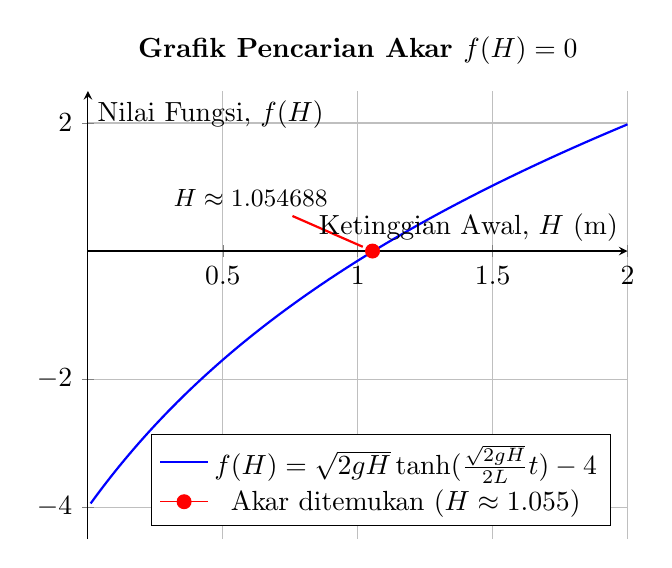
\begin{tikzpicture}
    \begin{axis}[
        title={\textbf{Grafik Pencarian Akar $f(H)=0$}},
        xlabel={Ketinggian Awal, $H$ (m)},
        ylabel={Nilai Fungsi, $f(H)$},
        xmin=0, xmax=2,          % Batas sumbu x sesuai interval bisection
        ymin=-4.5, ymax=2.5,      % Batas sumbu y
        grid=major,              % Menambahkan grid
        legend pos=south east,   % Posisi legenda
        axis lines=middle,       % Sumbu x dan y bertemu di (0,0)
        ]
        
        % 1. Plot fungsi f(H)
        % f(H) = sqrt(19.62*H) * tanh(3 * sqrt(19.62*H) / 10) - 4
        \addplot[
            domain=0.01:2,   % Domain H dari 0.01 (hindari H=0) hingga 2
            samples=100,     % Jumlah titik sampel untuk kehalusan kurva
            color=blue,
            thick
        ] {sqrt(19.62*x) * tanh(3 * sqrt(19.62*x) / 10) - 4};
        \addlegendentry{$f(H) = \sqrt{2gH}\tanh(\frac{\sqrt{2gH}}{2L}t) - 4$}

        % 2. Tandai titik akar yang ditemukan oleh metode bisection
        % Nilai H = 1.054688 dari tabel iterasi Anda
        \addplot[
            mark=*,
            color=red,
            mark size=2.5pt
        ] coordinates {(1.054688, 0)};
        \addlegendentry{Akar ditemukan ($H \approx 1.055$)}
        
        % 3. Tambahkan anotasi/label untuk titik akar
        \node[pin={[pin edge={red, thick}]135:{\small$H \approx 1.054688$}}] at (axis cs:1.054688, 0) {};

    \end{axis}
\end{tikzpicture}
\caption{Visualisasi pencarian akar dari fungsi $f(H)$ pada interval $[0, 2]$}
\label{fig:grafik_bisection}
\end{figure}

Perhitungan dengan rumus bernoulli dilakukan untuk memvalidasi hasil perhitungan numerik \textit{bisection method} dengan rumus:
\begin{equation}
v = \sqrt{2gH} \tanh\left(\frac{\sqrt{2gH}}{2L}t\right)
\end{equation}
Dengan memasukkan nilai-nilai yang telah ditetapkan:
\begin{equation}
v = \sqrt{2 \cdot 9.81 \cdot 1.054688} \tanh\left(\frac{\sqrt{2 \cdot 9.81 \cdot 1.054688}}{2 \cdot 5} \cdot 3\right)
\end{equation}
\begin{equation}
v = \sqrt{20.68} \tanh\left(\frac{\sqrt{20.68}}{10} \cdot 3\right)
\end{equation}
\begin{equation}
v \approx 3.9916 \, \text{m/s}
\end{equation}

Untuk menghitung galat relatif antara kecepatan target dan kecepatan yang dihasilkan dari perhitungan bernoulli, kita dapat menggunakan rumus:
\begin{equation}
\epsilon_r = \left| \frac{4 - 3.9916}{4} \right| \times 100\%
\end{equation}
\begin{equation}
\epsilon_r = \left| \frac{0.0084}{4} \right| \times 100\% \approx 0.21\%
\end{equation}

Hasil perhitungan dari \textit{bisection method} menunjukkan bahwa nilai ketinggian awal air ($H$) adalah \textbf{1.054688 meter} untuk mendapat nilai kecepatan aliran air sebesar $4.00 \, \text{m/s}$ dengan galat relatif sebesar \textbf{0.74\%} untuk nilai ketinggiannya. Dengan ketinggian yang sama, hasil perhitungan bernoulli menunjukkan bahwa kecepatan aliran air yang dihasilkan adalah sekitar $3.9916 \, \text{m/s}$ galat relatif antara kecepatan target ($4 \, \text{m/s}$) dan kecepatan yang dihasilkan ($3.9916 \, \text{m/s}$) adalah sekitar $0.21\%$. \\

\section{KESIMPULAN}
Dengan menggunakan \textit{bisection method}, hasil dari ketinggian awal air ($H$) yang diperlukan untuk mencapai kecepatan aliran $4 \, \text{m/s}$ adalah sekitar 1.054688 meter dengan galat relatif sebesar $0.74\%$. Perbandingan dengan hasil perhitungan bernoulli menunjukkan bahwa kecepatan aliran yang dihasilkan adalah sekitar $3.9916 \, \text{m/s}$ dengan galat relatif antar kecepatan perhitungan bernoulli dengan kecepatan target sebesar $0.21\%$ yang menunjukan persenan error sangat kecil hingga dibawah 1\%. Hal ini menunjukkan bahwa \textit{bisection method} adalah metode yang efektif untuk mencari akar dari fungsi non-linear dalam konteks aliran fluida. \\

\section{LINK GITHUB}
Berikut adalah link GitHub:
\url{https://github.com/BonifasiusRaditya/FinproKomputasiNumerik.git} \\

\section{LINK YOUTUBE}
Berikut adalah link YouTube:
\url{https://youtu.be/AHNSWor2pdk} \\

\begin{thebibliography}{00}
\bibitem{ref1} F. M. White, \textit{Fluid Mechanics}, 8th ed. New York: McGraw-Hill Education, 2016.
\bibitem{ref2} S. C. Chapra and R. P. Canale, \textit{Numerical Methods for Engineers}, 7th ed. New York: McGraw-Hill Education, 2015.
\bibitem{ref3} J. D. Anderson, \textit{Computational Fluid Dynamics: The Basics with Applications}, 2nd ed. New York: McGraw-Hill Education, 1995.
\bibitem{ref4} E. Kreyszig, \textit{Advanced Engineering Mathematics}, 10th ed. New York: Wiley, 2011.
\end{thebibliography}
\vspace{12pt}

\end{document}